
\iffalse
Features  
\begin{itemize}
	\item Qualitative representation - states and transitions
	\item State identification services:
	\begin{itemize}
		\item State details and attribute highlighting - histograms + attribute colors
		\item \lstopar{Timeline + parallel coordinates \cite{parcoords} - when do states occur in time}
		\item \lstopar{Coloring states based on attributes}
		\item Decision trees + rule extraction - Explanation of states
		\item Automatic name generation
		\item Zooming into a state + showing paths from a state
	\end{itemize}
\end{itemize}
\fi

\dunja{This needs a one sentence intro on the overall user interface.}
The system supports multiple users with datasets and precomputed models (as well as the ability to store new models in the system). Data is generally uploaded via CSV files.  Configuration consists of choice of desired attributes,  clustering method, aggregation strategy and attributes used to model transitions. The model is then constructed and the user can begin interactive exploration. The construction time varies depending on the size of 
their dataset and configuration. We conducted an experiment to test the performance of our \lstopar{methodology},
presented in section \ref{sec:implementation}.

The interface displays the model using a three panel user interface, an example of
which is shown in Figure \ref{fig:teaser} \lstopar{[TODO teaser reference not appearing]}. The central panel visualizes the model at the current scale as a graph. A state is represented by a circle  whose size represents the time/probability spent in the state, which is computed from the stationary distribution of the Markov chain. The transitions are represented by arrows, where again size represents the empirical transition probability. 

The computed model may be used as a monitoring tool, mapping incoming data onto the model in real-time. 
In this mode, the current state (green) and the most likely future states (blue)
are highlighted. The current state is determined by assigning a sample to its nearest 
centroid, as presented in Section \ref{sec:multiscale-implementation}, and is updated in real-time as
data arrives into the system.

The model is initially presented on a coarse scale with only a handful
of states. Users can then explore the model by either traversing the scales using the zoom 
function, as well as isolate and explore individual states using the ``Zoom Into'' function, \lstopar{or explore the 
graph as a tree using the ``Show Path'' function}.

Visualizing a Markov chain as a graph may not be, in itself,  sufficiently informative. The system offers several 
visualizations which assist users in identifying the meaning of states. These range from automatic
state naming, state histograms, attribute highlighting and timeline histograms to decision trees
which visualize the states' properties in a hierarchical manner and \lstopar{extracted rules}.
These services are shown when the user clicks on and selects a state. We describe these visualizations below.  For an overview of this functionality, see the supplementary material. The examples and the live system are available for testing at \url{http://streamstory.ijs.si} - see supplementary material for details. 

%and each transition with an arrow on the 
%central panel. The size of a state is calculated from the associated entry in the stationary distribution
%and is proportional to the fraction of time the system spends in the state. The thickness of each arrow
%is proportional to the associated transition probability. 

% The computed 
% When using the model as a
% monitoring tool, 
%After registering, the user is presented with a dashboard, where they can organize their models.
%If they wish to create a new model, they have to upload a CSV file with the dataset they would
%like to visualize. 
%They are then taken through a configuration form, where they select attributes,
%clustering method, aggregation strategy and attributes used to model transitions. When completing
%the form, their new model is constructed. 

%Once constructed, a StreamStory 

\subsection{Probability Distributions and Attribute Highlighting}

The most basic exploratory tool to help a user is to plot the distribution of data inside each state in the form of a histogram. When clicking on a state, the histograms of all the attributes are shown in the right-side panel like in Figure \ref{fig:teaser} \lstopar{[teaser not showing!]}. Context for each distribution is shown as a global distribution of that attribute in the background.

%
%To assist the users to distinguish between states, we highlight each attribute either green of red.
%The color is chosen based on how typical the attribute is for the state. 
To help users understand the  values of attributes within a state, the attributes are colored according to their typical values.  For example, a bright green
value indicates that the attribute typically  has a higher value in this state compared to other states, while
a bright red color suggests, this value is low compared to other states. An example of attribute 
highlighting can be seen in Figure \ref{fig:example-naming-histogram}.

The color is calculated in the initialization step by first classifying all the samples assigned to this state 
against samples assigned to other states using a logistic regression model. \lstopar{The features used in the 
classification are all the dimensions of the input signal, which correspond to all possible attributes.}
The final color is determined by extracting weights from the models and associating positive weights
with green and negative with red.

The users can also view the distribution of attributes across states, by selecting a specific attribute.
When doing so, the states are recolored based on the value of the selected attribute - again, green indicates
a high value, while red indicates a low value.

%%here

\subsection{Automatic State Labeling}

Abstract states are often uninformative. While the transitions between states gives us insight into the dynamics of the system, it fails to provide a comprehensive summary 
of the dataset. Our initial user evaluations showed that first time, non-technical users had difficulty interpreting unlabeled states. % and had difficulty executing even the simplest tasks like finding
%states with high temperature in example \ref{sec:experiments-weather}}.

To help alleviate this, the system provides an automatic, data-driven, naming service. The service labels states using $<attribute,value>$ pairs based on the inner-state distribution of attributes. The attribute is selected as one of the input signals, while the value is a discrete level with values: lowest, low, mean, high and highest. \primoz{this sentence isnt clear} \lstopar{Better now?}

Both the attribute and the level used in the label are computed by comparing the inner-state attribute
distributions to the global attribute distributions. The attribute selected by the naming process is
the one with the lowest $p$-value of the inner-cluster $40$-th and $60$-th percentile. The level is
then determined according to the $p$-value. If the $p$-value is below $0.12$ the attribute is labeled
as lowest or highest, while if the $p$-value is below $0.25$ it is labeled low or high. If none of the
attributes achieve a $p$-value of $0.25$ the state is labeled as a mean state. An example of an automatic
label, along with the associated inner-state and global histogram is shown in Figure \ref{fig:example-naming}.

\begin{figure}[h!]
	\centering
	\begin{subfigure}{.48\columnwidth}
	  	\centering
	  	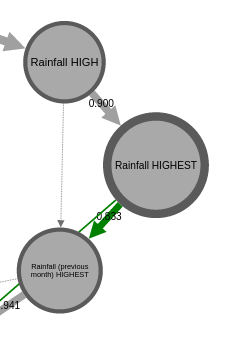
\includegraphics[width=0.7\columnwidth]{example-state-naming}
  		%\caption{\label{fig:example-naming-label}\lstopar{TODO}}
	\end{subfigure}
	\begin{subfigure}{.48\columnwidth}
	  	\centering
	  	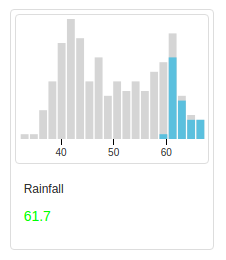
\includegraphics[width=\columnwidth]{example-state-naming-histogram}
	  	%\caption{\label{fig:example-naming-histogram}\lstopar{TODO}}
	\end{subfigure}
	\caption{Example output of the automatic state labeling service shown on the weather dataset presented in Section \ref{sec:experiments-weather}. The system labeled the bold state on the left hand side as "Rainfall HIGHEST", matching the inner-state distribution of rainfall shown on the right hand side.}
	\label{fig:example-naming}
\end{figure}

\iffalse
In order to assist the user in identifying the meaning of states, the system provides automatic default
state names, based on the distribution of attributes in the state. Each state is given a default name
by combining its most outstanding attribute with a discrete level: LOWEST, LOW, HIGH or
HIGHEST.

The attribute and the level are chosen by comparing its distribution inside the state to the global
distribution in all the states through histograms. This is achieved by first computing the percentiles
of the global distribution. The $40^{th}$ percentile is then computed for the state distribution and
compared against the global distribution. If this percentile lies below the $25^{th}$ or $12^{th}$
percentile, the state is marked with LOW or LOWEST respectively. The final name is chosen according
to the attribute which lies in the lowest percentile.
\fi

\subsection{Decision Trees and Rule Extraction}

An alternate description of states is generated through decision trees~\cite{Witten:2005:DMP:1205860}. Decision
trees are classification models often used in domains such as medicine for their explanatory power.
When a decision tree is induced, a splitting attribute and cut value are chosen recursively by a
design time criteria. The user can then interpret the tree by traversing the path from the root 
to one of the leafs.

Decision trees are provided as another tool for explaining states. We compute one tree for each
state by classifying the observations of the state against the observations of all other states,
obtaining a quantitative description of the state. We then extract rules from the decision tree,
providing a short summary of the state in the form of $A_i > t_i \cup A_j \in (t_{j_1}, t_{j_2}]$.

Figure \ref{fig:example-decision-tree-and-rule} show an example decision tree and extracted rules
from a state in the weather dataset presented in section \ref{sec:experiments-weather}.

\begin{figure}[h!]
	\centering
	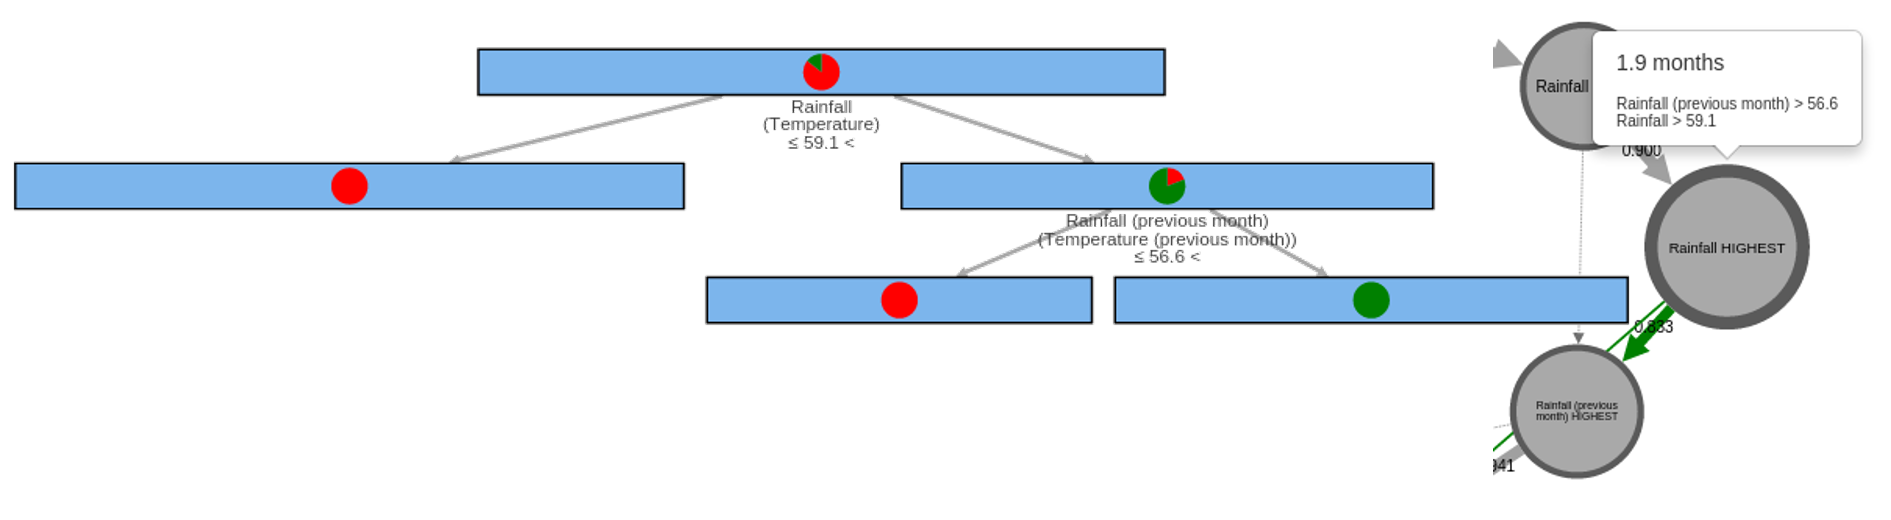
\includegraphics[width=\columnwidth]{example-tree-rule}
	\caption{Example output of a decision tree (left) and a rule (right) describing a state in the weather dataset presented in Section \ref{sec:experiments-weather}. We can see that the system describes the state as having rainfall over $59.1 mm$ and the previous month rainfall over $56.6 mm$.}
	\label{fig:example-decision-tree-and-rule}
\end{figure}

\subsection{Streaming Data}
The system is also able to visualize streaming data based on a precomputed model. Given a training set, the multiscale model is built. The system can then process the streaming data. For each new point, it determines its current state using on a nearest neighbor search to the centroids of the states. This is done at all scales, allowing the user to visualize the current state and possible next states at different levels interactively. The system allows for alarms to be set to detect when the system enters a particular state or when the probability of entering a paraticular state exceeds some threshold. The probabilities are computed based on the Markov model at the scale at which the alarm is set 
(see Supplementary Video).

\iffalse
\begin{figure}[h!]
	\centering
	\begin{subfigure}{.3\columnwidth}
	  	\centering
	  	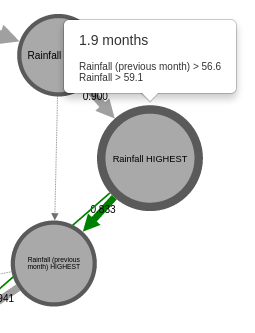
\includegraphics[width=\columnwidth]{example-rule}
%  		\caption{\lstopar{TODO}}
  		\label{fig:example-rule}
	\end{subfigure}
%	\begin{subfigure}{.68\columnwidth}
	\begin{subfigure}{0.9\columnwidth}
	  	\centering
	  	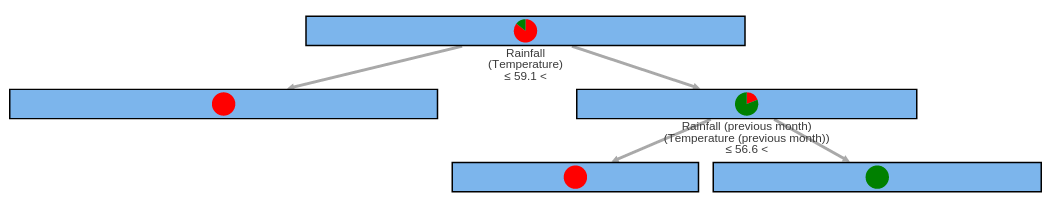
\includegraphics[width=\columnwidth]{example-decision-tree}
%	  	\caption{\lstopar{TODO}}
	  	\label{fig:example-decision-tree}
	\end{subfigure}
	\caption{Example output of a decision tree (right) and a rule (left) describing a state in the weather dataset presented in Section \ref{sec:experiments-weather}. We can see that the system describes the state as having rainfall over $59.1 mm$ and the previous month rainfall over $56.6 mm$.}
	\label{fig:example-decision-tree-and-rule}
\end{figure}
\fi

\iffalse

\subsection{Visual Assistance}

When a state becomes selected, the user interface presents the user with several visual aids which
assist them in identifying the states' meaning. The first of these aids is the timeline histogram
which shows the distribution of the states occurrence over time. An example is shown in Figure 
\ref{fig:time-hist}.

\begin{figure}[h!]
	\centering
	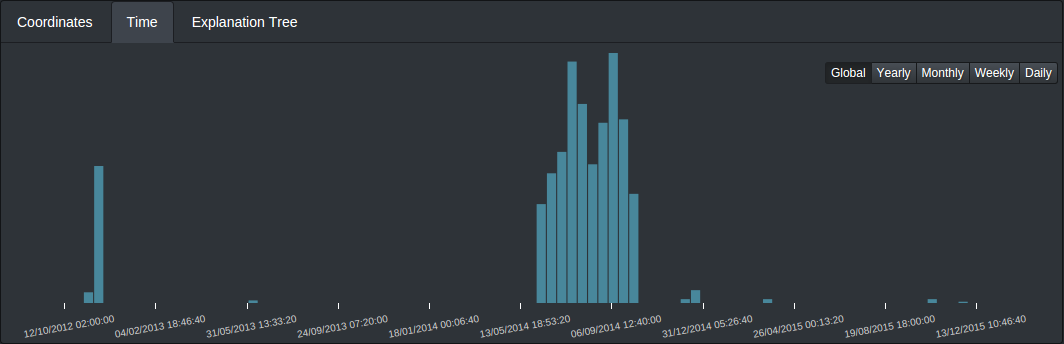
\includegraphics[width=\columnwidth]{timeline}
	\caption{[TODO example decision tree].}
	\label{fig:time-hist}
\end{figure}

This provides several common time scales (e.g. hourly, daily, weekly, yearly, etc.). This can help identify periodic or cyclic behaviour in the data. 

\primoz{more on decision trees, arbitrary time scales}
[TODO histograms]
\fi
